\documentclass[tikz,border=2pt]{standalone}
\usepackage{amsmath,amssymb}
\usepackage{tikz}
\usetikzlibrary{arrows.meta,calc}

\begin{document}
% Orthogonal projection onto the line through u = (2,1): P v is the foot of the perpendicular
% from v, and projecting again changes nothing (P^2 = P).
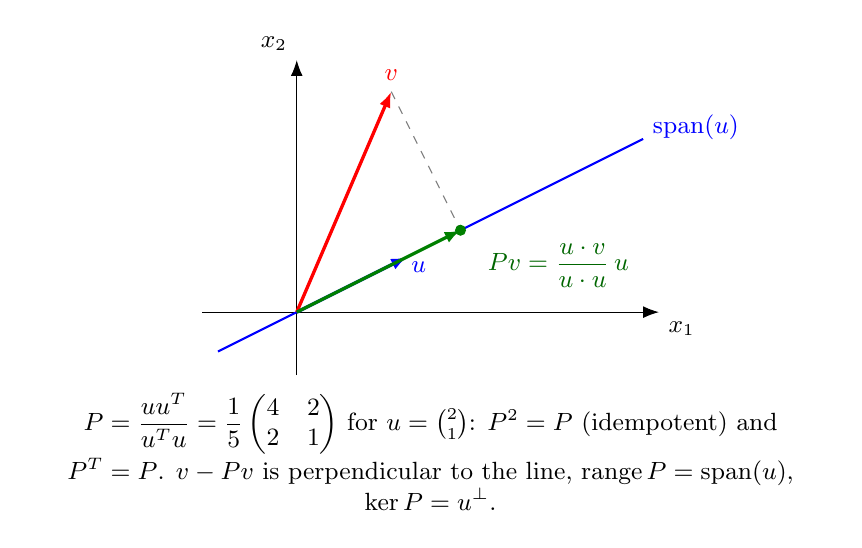
\begin{tikzpicture}[every node/.style={font=\small}, >={Latex[length=2mm]}]
	\draw[->] (-1.2,0) -- (4.6,0) node[below right] {$x_1$};
	\draw[->] (0,-0.8) -- (0,3.2) node[above left] {$x_2$};
	\draw[blue, thick] (-1.0,-0.5) -- (4.4,2.2);
	\node[blue, anchor=west] at (4.4,2.35) {$\operatorname{span}(u)$};
	\draw[->, blue, very thick] (0,0) -- (1.4,0.7) node[below right, inner sep=1pt] {$u$};
	\coordinate (V) at (1.2,2.8);
	\coordinate (PV) at ($ {(1.2*2+2.8*1)/5}*(2,1) $);
	\draw[->, red, very thick] (0,0) -- (V) node[above] {$v$};
	\draw[dashed, gray] (V) -- (PV);
	\draw[->, green!50!black, very thick] (0,0) -- (PV);
	\fill[green!50!black] (PV) circle (2pt);
	\node[green!40!black, anchor=north west, inner sep=2pt] at (2.35,0.95) {$Pv=\dfrac{u\cdot v}{u\cdot u}\,u$};
	\node[anchor=north, align=flush center, text width=10cm] at (1.7,-0.9) {$P=\dfrac{uu^{T}}{u^{T}u}=\dfrac15\begin{pmatrix}4&2\\2&1\end{pmatrix}$ for $u=\binom21$: $P^2=P$ (idempotent) and $P^{T}=P$. $v-Pv$ is perpendicular to the line, $\operatorname{range}P=\operatorname{span}(u)$, $\ker P=u^{\perp}$.};
\end{tikzpicture}
\end{document}
